\chapter{Interpretation of Morphogen Gradients by a Bistable Circuit}
\label{chapter:double-exclusive}
\epigraph{\textit{memory of younger days}}{Ocarina of Time}
\section{Preface}
\subsection{Problem Statement \& Context}

\begin{enumerate}
    \item Keep focus on developmental biology
    \item Revised supplement as this chapter
\end{enumerate}

\usetikzlibrary{patterns}
\begin{Figure}
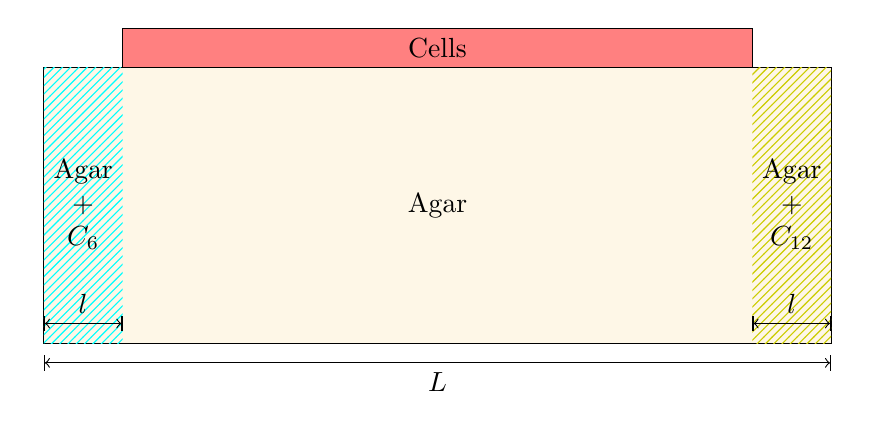
\begin{tikzpicture}
\def\H{3.5}
\def\L{10.0}
\def\l{1.0}
\def\epsilon{0.5}
\def\dx{0.25}
\def\dy{0.25}

%cell region
\filldraw[fill=Red!50!white] (\l,\H) rectangle (\L-\l,\H+\epsilon) node[midway] {Cells};

%agar region
\filldraw[fill=Dandelion!10!white,draw=black] (0,0) rectangle (\L,\H) node[midway] {Agar};
\fill[pattern=north east lines, pattern color=cyan] (0,0) rectangle (\l,\H) node[midway] {\begin{tabular}{c}Agar\\+\\$C_6$\end{tabular}};
\fill[pattern=north east lines, pattern color=yellow!80!black] (\L-\l,0) rectangle (\L,\H) node[midway] {\begin{tabular}{c}Agar\\+\\$C_{12}$\end{tabular}};
\draw[|<->|](0,-\dy) -- (\L,-\dy) node[midway, below] {$L$} ;
\draw[|<->|](0,\dy) -- (\l,\dy) node[midway, above] {$l$} ;
\draw[|<->|](\L-\l,\dy) -- (\L,\dy) node[midway, above] {$l$} ;
%\draw[|<->|](\L+\dx,0) -- (\L+\dx,\H) node[midway, right] {$H$} ;
%\draw[|<->|](\L+\dx,\H) -- (\L+\dx,\H+\epsilon) node[midway, right] {$H_\varepsilon$} ;

%axis
%\draw[->] (-\dx-\dy,-\dy)--(0.1*\L,-\dy) node[right] {$x$};
%\draw[->] (-\dx,-\dx-\dy)--(-\dx,0.5*\H) node[above] {$y$};
\end{tikzpicture}
\caption{Geometry of opposing gradients experiment}
\label{fig:experiment_geometry}
\end{Figure}

This section outlines how the Design---Learn pipeline may help achieve a specific
aim in a typical collaboration between theory, computation and experiment.
The aim of this project is to reconstitute and control minimal self-organisation
mechanisms which are believed play crucial roles in developmental biology. To this
end \textit{E. Coli} has been genetically engineered to produce orthogonal responses
to two different input signals --- henceforth this organism will be referred to as the
\textit{double exclusive reporter} circuit \cite{Grant2016}. The colony of reporters
serve as a reduced model for a multi-cellular organism during embryonic stages of
development. While patterns with sharp boundaries have successfully been realised,
producing Turing instabilities remains challenging as the system needs to be such
that patterns develop before the colony reaches stationary phase.
The role of theory and computation in this project is to help identify the
parameter regimes that produce controllable and self-organised patterns.

\subsection{Contributions}

\textbf{Grisha Szep} is co-second author with \textbf{Om Pantage}. \textbf{Paul Grant}, \textbf{Neil Dalchau}, \textbf{Jacob Halatek} and \textbf{Andrew Philips} conceived and designed the study. \textbf{Paul Grant} designed and built the genetic circuits. \textbf{Paul Grant}, \textbf{Om Pantage} and \textbf{Valerie Coppard} performed the experiments. \textbf{Grisha Szep}, \textbf{Jacob Halatek} and \textbf{Neil Dalchau} conceived and implemented theory and modelling and wrote the supplementary information. All authors analysed and interpreted the data. \textbf{Paul Grant} and \textbf{Andrew Philips} wrote the main text. All authors provided input into the manuscript. The contributions of \textbf{Grisha Szep} the main text and supplementary include:
\begin{itemize}
    \item \textbf{Figure 1.b} Spatial simulations of parameterized model
    \item \textbf{Figure 2.a-b} Calculation of region of bistability predicted by the parameterized model using arc-length continuation algorithms
    \item \textbf{Figure 3.b-e} Wrote bespoke inference code for quantification of boundary velocity from microscopy movies and comparison to theoretical model
    \item \textbf{Figure 4.d-e} Spatial simulations of the parametrized model. Novel state-space analysis of boundary formation and bistability
    \item \textbf{Figure S10.c} Spatial simulations analysed in state-space
    \item \textbf{Figure S13} A novel method for quantifying hysteresis in the flow cytometry experiments as population separation
    \item \textbf{Figure S25-S26} Bistability analysis of parametrized models and comparison to qualifications from flow cytometry
    \item \textbf{Figure S27-S33} Simulations of boundary velocity, novel way of understanding them in state space and bespoke inference methods for quantification of boundary velocity from microscopy movies
    \item \textbf{Figure S36} State space geometry for model with feedback loops
    \item \textbf{Supplementary Sections 2.2-2.4} Wrote sections outlining the methods for extracting bistability regions from data and models with and without feedback loops
    \item \textbf{Movies 1-5} Simulations of expression boundary formation
    \item \textbf{Code} Released code with documentation in \href{https://github.com/gszep/double-exclusive-reporter}{GitHub Repository}
\end{itemize}

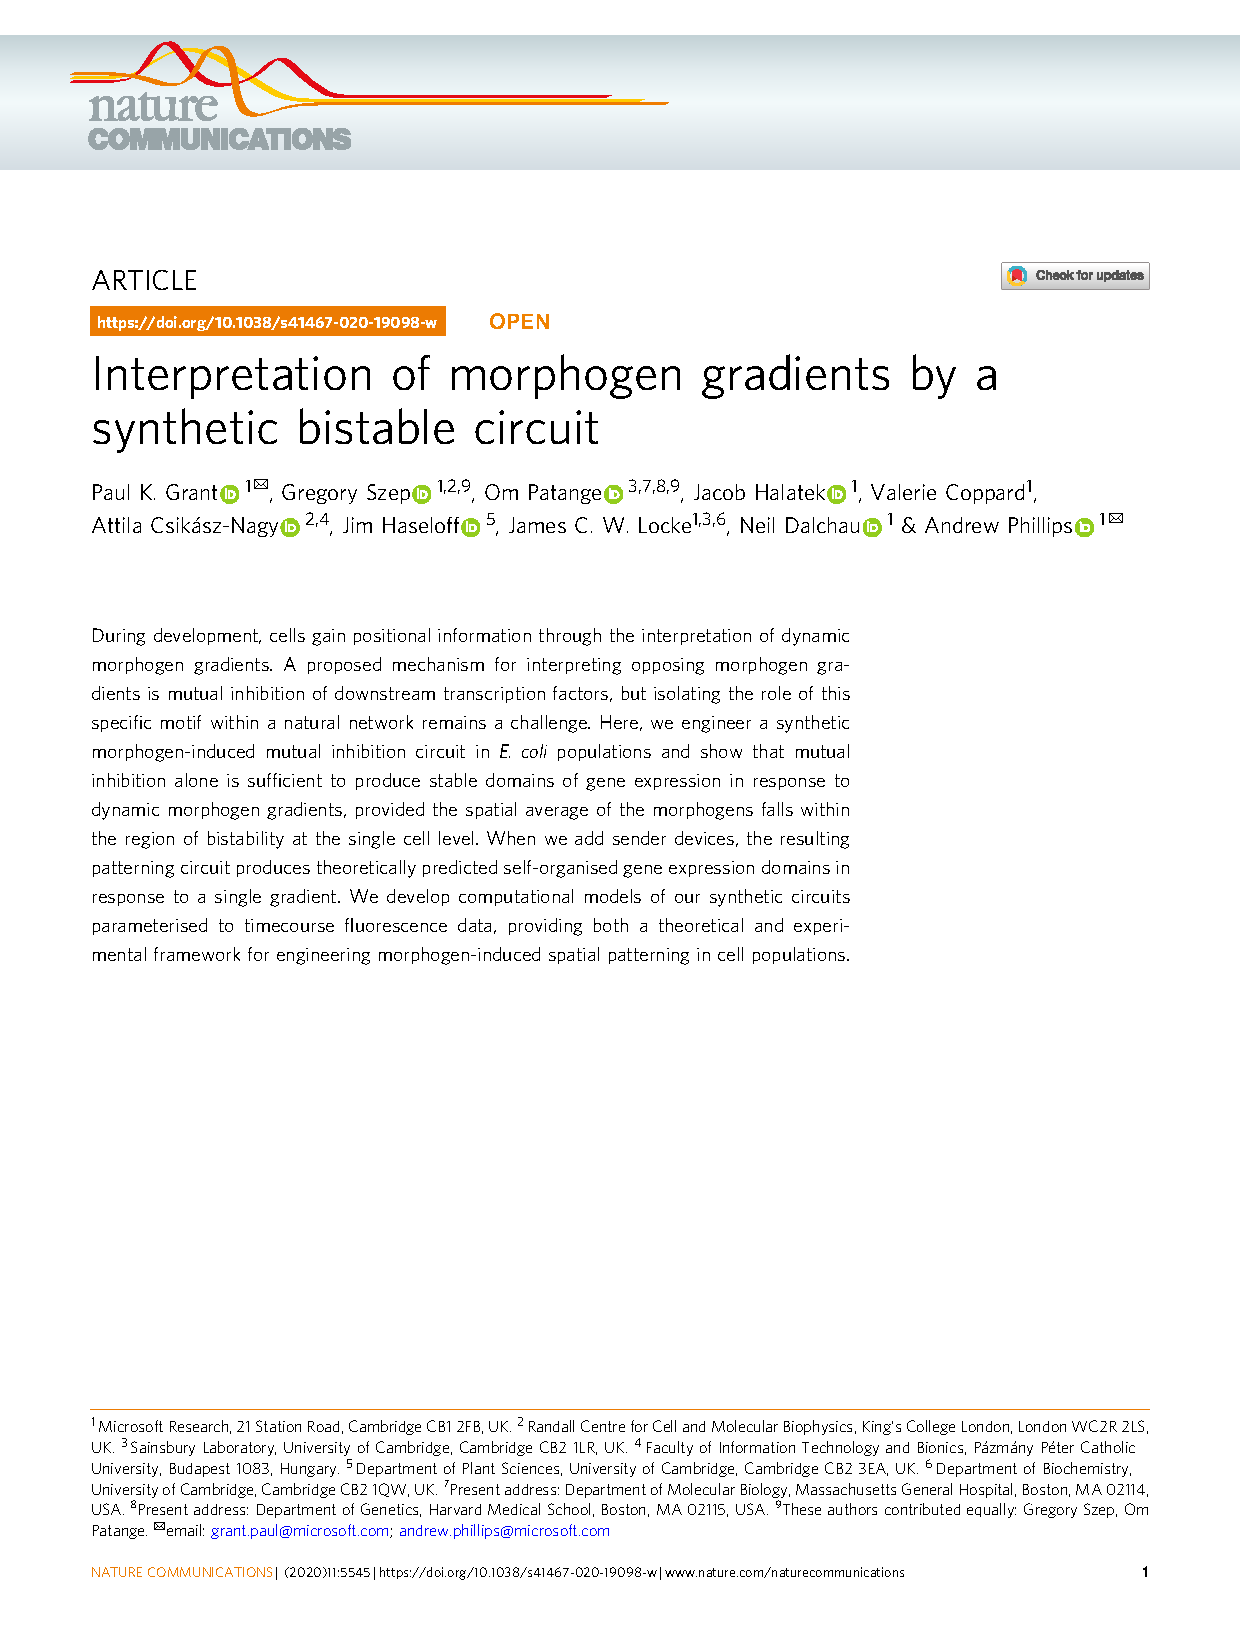
\includepdf[pages=1-8, offset=75 -90, scale=0.85, frame,
        clip,trim=10mm 5mm 10mm 0mm,
        pagecommand={}, addtotoc={
        1,section,1,Abstract,double-exclusive:abstract,
        2,section,1,Introduction,double-exclusive:introduction,
        2,section,1,Results,double-exclusive:results,
        2,subsection,2,Engineering mutual exclusivity,double-exclusive:exclusivity,
        3,subsection,2,Mutual inhibition results in bistability,double-exclusive:bistability,
        4,subsection,2,Hysteresis produces stable boundaries,double-exclusive:boundaries,
        4,subsection,2,A secondary gradient creates self-organised domains,double-exclusive:self-organisation,
        5,section,1,Discussion,double-exclusive:discussion,
        6,section,1,Methods,double-exclusive:methods,
        6,subsection,2,Plasmid construction,double-exclusive:plasmids,
        6,subsection,2,Plate fluorometer assay,double-exclusive:plates,
        6,subsection,2,Flow-cytometric analysis of hysteresis,double-exclusive:flow,
        7,subsection,2,Microfluidics,double-exclusive:microfluidics,
        7,subsection,2,Microfluidics microscopy,double-exclusive:microscopy,
        7,subsection,2,Solid culture assays,double-exclusive:cultures},
    addtolist={
        2, figure, {\textit{Fig. 1}\quad A synthetic gene circuit for morphogen interpretation.}, fig:double-exclusive:overview,
        3, figure, {\textit{Fig. 2}\quad Mutual inhibition produces bistability.}, fig:double-exclusive:bistability,
        5, figure, {\textit{Fig. 3}\quad Formation of stable boundaries.}, fig:double-exclusive:boundaries,
        6, figure, {\textit{Fig. 4}\quad Addition of a Relay circuit creates self-organised domains of gene expression.}, fig:double-exclusive:relay
}]{publications/double-exclusive.pdf}

\section{Afterword}

The decision to focus on single cell trajectories and flow cytometry came from the limitations of using microplate data in Chapter \ref{chapter:double-exclusive}. The model parameters $\theta$ were estimated using a hierarchical monte-carlo approach and time-course fluorescence microplate measurements (details of which can be found in Appendix \ref{appendix:double-exclusive:inference}). The time-courses include information about dynamical transients and colony growth in liquid culture. The desired cusp bifurcation, however, lives in state-space rather than the time-domain. The disconnect between the domain that the data lives in and the domain of the design goals poses the risk of over-fitting the model on undesired information that exists in the data domain. 

It is not possible to observe the cusp bifurcation in microplate data, due to the averaging of signals originating from heterogeneous cell populations. Instead, the cusp bifurcation can be observed in flow cytometry measurements of colonies in exponential phase (Supplementary Figure \ref{fig:double-exclusive:flow-hysteresis}) and microfluidic fluorescence microscopy data (Figure \ref{fig:double-exclusive:bistability}c) where computations on single-cell trajectories reveal the hysteresis loop which must necessarily accompany the cusp. 